\section{Računalniška znanost in programiranje}
\label{sec:računalniška_znanost_in_programiranje}

Računalniška znanost ima številne različice definicij, v grobem jo
lahko definicijo strnemo v naslednjih trditvah \cite{guideTCS}.

\begin{itemize}
\tightlist
\item Ukvarja z značilnostmi tisktega kar je izračunljivo.
\item Je znanost, ki izhaja iz več področij in ime korenine v matematiki,
znanosti in inženirstvu.
\item Ima mnoga podpodročja in je interdisiplinarna z biologijo,
ekonomijo, medicino, zabavo.
\item Ime računalništvo ali računalniška znanost nas lahko tudi zavede in
jo zamenjamo z področjem uporabe računalnika.
\end{itemize}

%Še je potrebno dodati kakšno definicijo z druge literature.

\subsection{Zgodovina programskih jezikov}
\label{sec:zgodovina_programskih_jezikov}


%Splošna zgodovina uporabe računalništva v izobraževanju
%Razdeljeno imam zgodovino rac. v izobrazevanju in programiranje v
%izo, ali je naj vse skupaj. Na kratko dodaj računalniška obdobja, kot
%jih je predstavil Gerlič

Uporaba računalništva v izobraževanju je bila deležna številnih
sprememb. Sama uporaba računalnika v izobraževanju je tesno povezana z
razvojem računalnikov.  Začetno obdobje, 1960 letih prejšnjega
stoletja so računalniki bili zelo dragi in veliki glavni računalniki (
\emph{ang. mainframe} ), na njih se je učilo programiranja, a so se
uporabljali tudi za druga področja.  V tem obdobju se je za učenje
programiranja uporabljal \textbf{FORTRAN} ali
\textbf{asembler}. Programi so bili majhi in enostavi, zaradi fizičnih
omejiteh takratnega delovnega pomnilnika. Temu začetnemu obdobju pravimo
\textbf{terminalsko obdobje} \cite{gerlic_2000}.

V 1970 so na trg prišli manjši računalniki, ki so bili tudi cenejši in
zmogljivejši. V tem času pride v ospredje strukturirano programiranje.
Najpopularnejši programski jezik je bil \textbf{PASCAL}. Predstavnimi
obdobja \textbf{mikroračunalnikov} so bili \emph{Commodore 64,
  Sinclare ZX-81, Apple II}.

V 1980 so se prvič pojavili \textbf{samostojni osebni računalniki}. Programski
jeziki v tem obdobju so bili strukturirani in močnega tipa (
\emph{ang.  strong type.} ). Med te spada \textbf{Ada, Modul 2, ML in
  naj omenimo še Prolog}.

V naslednjem desetletji, 1990 so v ospredje prišli objektno
orjentirani programski jeziki, kot sta \textbf{C++} in \textbf{JAVA}
\cite{thesisAWebP}.

% //Umestitev računalnik v izobraževanju na primarnem področju.
% -\textgreater{} Gerlič Uporaba računalika v namene učenje računalništva
% in programiranja.

% //Doodaj generacije programskih jezikov. //Dodaj vrste programskih
% jezikov.

Metode poučevanja računalništva so se prav tako spreminjale. 1960 so
računalnike uporabljali samo za poučevanje programiranja. Povdarek pri
predmetih programiranja je bil predvsem na detaljlih zmožnosti
programskega jezika. Programiranje je bilo omejeno le na reševanje
enostavnih primerov in poudarka na splošnem reševanju problemov ni
bilo.

V 1970 je reševanje problemov in abstrakcija podatkov postala glavni
in najpomembnejši del vseh programerskih predmetov, kar velja še
danes. Programi so postali večji, bolj interaktivni in spremenil se
je vnos podatkov z tekstovnega v grafičnega. Vsebina predmetov
računalništva se je hitro razširjala, kakor so se množili številni
programski jeziki \cite{thesisAWebP}.

Posebno mesto v izobraževanju ima programski jezik
\textbf{LOGO}. Z ekipo ga je Seymour Papert. Značilnost programskega
jezika je ta, da z programsko kodo rišemo grafiko, ki jo lahko
predstavimo na zaslonu ali z \emph{``z želvo''}, ki se premika po tleh
z ukazi in riše sliko na podlago. Programski jezik je bil prvič
zasnovan v namene učenja programiranja.

%Dodaj slike logo + želva!

% \begin{figure}[h!]
%   \centering
%     \includegraphics [width=1\linewidth, keepaspectratio =
%    1] {./images/?}
%    \caption{Niem našel primerne slike!}
%    \label{fig:logo}
%  \end{figure}

 
\subsection{Osnovni pojmi}
\label{sec:kaj_je_programiranje}

%% Splošne definicije programiranja.
%% Ni le pisanje kode temveč tudi uspešno reševanje nalog in
%% problemov?

Preden nadaljujemo moramo razjasniti nekaj osnovnih pojmov, ki se
pojavljajo računalniški znanosti.

\subsubsection{Program}
\label{sec:program}

Računalniški program je zbirka navodil, ki opravlja točno določeno
nalogo in jo izvajamo na računalniku. \textbf{Centralno procesna
  enota} je tista, ki izvajanje programa omogoča. Računalniški program
navadno napiše \textbf{programer} v nekem \textbf{programskem jeziku},
postopku pisanja programa pravimo \textbf{programiranje}. Programski
jezik omogoča, da je program zapisan v takšni obliki, da je berljiv za
ljudi in je zapisan v \textbf{izvorni kodi}. Da računalnik razume
napisan program, ga prevede \textbf{prevajalnik
  (\emph{ang. compiler})} v \textbf{strojno kodo} ali ga
\textbf{tolmači} tolmač.  
\cite{wiki:computer_program}.

\subsubsection{Algoritem}
\label{sec:algoritem}

Z besedo algoritem ponazarjamo postopek, ki je zgrajen iz posameznih
operacije, ki se izvajajo po posameznih korakih. Algoritem daje rešitev
za izračune, procesiranje podatkov, avtomatizacijo postopkov.
Ime besed \emph{``algoritem''} prihaja z imena \textbf{Al-Khwārizmī},
Perzijskega matematika, astronoma, geografa in učenjaka \cite{wiki:algorithem}.

Pri pregedu učnih načrtov v poglavju
\ref{sec:neobvezno_izbirni_predmet_rac} smo lahko zasledili cilje kot
so:

\begin{itemize}
\tightlist
\item \textbf{znajo vsakdanji problem opisati kot zaporedje korakov},
\item \textbf{znajo z algoritmom predstaviti preprosto opravilo},
\item \textbf{algoritem predstavijo simbolno (z diagramom poteka) ali s
  pomočjo navodil v preprostem jeziku}.
\end{itemize}

% Poglejmo nekaj primerov, kako lahko s pomočjo spletnih portalov za
% učenje programiranja zadostimo tem ciljem in kaktere informacije
% najdemo. Na strani \href{https://code.org}{code.org}. Podroben opis
% strani je v poglavju x.x. Algoritmov se učijo že najmlajši udeleženci
% zato si pri lažjem raumevanju pojma algoritem lahko pomagamo, z
% pristopom \textbf{računalništva brez računalnika}. Spodaj prikazujemo
% dva primera.

Prikazali bomo več različnih predstavitev algoritma, najprej bomo
rešitev zapisali v besedilni obliki, zatem bomo rešitev podali z
diagramom poteka, na koncu bomo rešitev podali še z programskim
jezikom Scratch in Python.  Za primer bomo prikazali primer algoritma,
ki reši naslednjo nalogo.

%Možnost programskih primerov v takem slogu.

%Dodaj diagram poteka!

\begin{examplebox}[label={prog:al01}]{Algoritem - Najdi največje število}
Algoritem med podanimi števili poišče največje število.

Postopek zapisan v \textbf{besedilu}:
\begin{enumerate}
\tightlist
\item Zapišemo si začetno število, naj bo $0$.
\item Števila v seznamu preglejujemo po vrsti.
\item Vsakič, ko najdemo večje število, ko je naše začasno število,
\item To začasno število prečrtamo in napišemo tisto z seznamoa, ki je
  večje.
\item Postopek ponavljamo, dokler ne pridemo na konec seznama.
\end{enumerate}


% Tu bi bilo dobro, da bi lahko prikazal tekst in sliko v eni vrsti.
Podprogram v \textbf{Scratchu}:

%\begin{figure}
    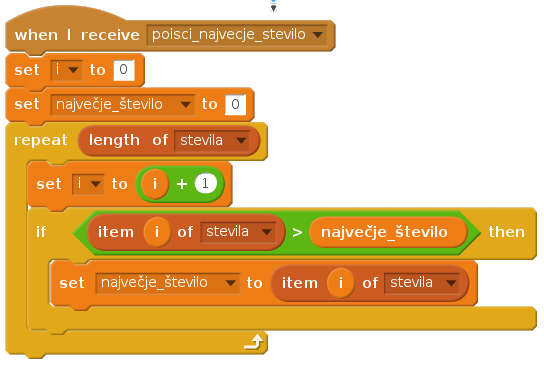
\includegraphics [width=0.6\linewidth, keepaspectratio =
    1] {./images/scratchImg/01-Scr_Alg-NajvecjeSt-img_trs.png}
    % \caption{Test}
    % \label{fig:scr:01-Alg_najdiNajvecje}
%\end {figure}

Podprogram v \textbf{Pythonu}:

\begin{lstlisting}[language=Python]
def najdiNajvecjeStevilo(seznam):
    """Funkcija poisce najvecje stevilo v seznamu."""
    i = 0
    najvecje_stevilo = 0
    for i in range(len(seznam)):
        if seznam[i] > najvecje_stevilo:
            najvecje_stevilo = seznam[i]
    return najvecje_stevilo
\end{lstlisting}
\end{examplebox}

\subsubsection{Programiranje in kodiranje}
\label{sec:programiranje_kodiranje}

Izraz programiranja smo že spoznali. Veliko krat slišimo tudi izraz,
\textbf{``kodiranje'' (\emph{ang. coding})}. Povedali bi lahko da
izraz pomeni, pisanje programske kode, konček izdelek, tisto kar na
koncu damo \textbf{prevajalniku}, kar je \textbf{izvorna koda}, da
prevede v \textbf{strojno kodo}, katero lahko potem zaganjamo.

Za vsakim programiranjem stoji seveda nek programer, lahko bi rekli,
da je za vsakim kodiranjem nekdo, ki mu pravimo
\textbf{koder}. Programer in koder stav veliko krat, dana v isti koš,
vendar si to čisto ne zaslužita, saj je programer, nekdo ki načrtuje
rešitve, na različne načine in z razčličnimi orodji preden sploh
zapiše kaj programske kode. Koder po drugi strani je tista oseba, ki
se dobro spozna na programske jezike vendar, dela veliko krat po
načrtu programera, je tisti ki na kocu zapiše rešitve in je pri tem
zelo unčikovita. Čeprav se ta dva poklica zelo povezana in so meje med
njima tudi veliko krat zabrisane sploh, če je programer in koder ena
in ista oseba \cite{web:coder}.

Pri samem poučevanju računalništva, lahko menimo, da je v prvi vrsti
pomembno to, da se učimo strategije reševanja problemov, mora
obstajati težnja kako poučevati, da bo čim več učencev postalo dobrih
programerjev in samo koderjev.

\subsubsection{Urejevalnik besedil}
\label{sec:urejevalnik_besedil}

Dober urejevalnik besedi lahko programerju lajša delo s številnimi
zmožnostmi. Opisali smo nekatere, saj nam bodo te pomagale lažje
prepoznati dober urejevalnik besedil.

%Podrobneje opiši zmožnosti urejevalnika besedil.

\begin{itemize}
\item \textbf{Barvanje rezerviranih besed prog. kode.} je značilno za
  skoraj vsak novo dobni urejevalnik besedil. Z različnimi barvami je
  olajšano branje programske kode.
\item \textbf{Samodejno zamikanje vrstic programske
    kode}. Urejevalnik, ki ima to zmožnost zna prepoznati, ko sledi
  nov del programske kode, ki je zamaknjen npr. za stavkom
  \texttt{if/else}.
\item \textbf{Ponujanje predlog za samo dokončevanje rezerviranih
    besed in funkcij prog. jezika}. Ob pisanju programske kode
  urejevalnik ponuja dokončevanje programske kode.
\item \textbf{Izpis opisa funkcij z atributi}. 
\item \textbf{Samodejno zaključevanje oklepajev}. Odprti oklepaj se
  samodejno zaključi z zaprtim in smernik za pisanje se postavi v
  sredino med oba oklepaja. 
\end{itemize}

\subsubsection{Integrirano razvojno okolje}
\label{sec:integrirano-raz-okolje}

Del \textbf{integriranega razvojnega okolja} (\textbf{IRO})
(\emph{ang. Integrated development environment \textbf{IDE}}) je dober
urejevalnik besedil, kot smo ga opisali v prejšnjem poglavju. Za IRO
je značilno, da omogoča \textbf{pisanje, testiranje, razhroščevanje}
in \textbf{prevajanje končnega programa}. Omogočajo povezavo med
datotekami projekta in knjižnicami. Svoje zmožnosti nadgrajujejo s
številnimi zunanjimi orodji, ki jih navadno vklopimo preko
vtičnikov. Slabost IRO je ta da so veliki programski paketi, ki včasih
znajo biti okorni in počasni. Pri nekaterih obsežnih IRO je tudi čas,
ki ga potrebujemo, da se ga naučimo uporabljati dolgotrajen.

\subsection{Programske paradigme}
\label{sec:programske_paradigme}

Paradigma je način kako obravnavamo in gledamo na stvari, je okvir v
katerem leži naša interpretacija realnosti sveta. Paradigma
najpogosteje pomeni vzorec delovanja v znanstvenem ali drugem
raziskovanju.  Izraz programske paradigme je več pomenka, ki povzema
mentalne procese, strategije reševanja problemov, povezave med
različnimi paradigmami, programske jezike, stil programiranja in še
več \cite{wiki:paradigme} \cite{guideTCS}.

%//Glavna definicija.
Programske paradigme so hevristike, ki se uporabljajo za reševanje
problemov. Programska paradigma analizira problem, čez specifičen
pogled in na ta način formulira rešitev za dani problem, ki ga razdeli
na manjše dele med katerimi definira razmerja.

Programske paradigme so na primer proceduralno, objektno orientirano,
funkcijsko, logično in istočasno programiranje. V nadaljevanju
spoznamo značilnosti programske paradigme objektnega programiranja,
saj je ta v zadnjih dve desetletjih najbolj razširjena. 

\subsubsection{Objektno orientirano programiranje}
\label{sec:objektno_orijentirano_programiranje}

%V objektno orientiranem \textbf{OO} pristopu programer raz

V objetno orientirano \textbf{OO} programiranje je način kako
programerji razmišljajo o svojem delu. Princip OO model realnosti
sveta predstavlja v \textbf{razredih \emph{ang. class}}. Z takim
načino zapisa programske kode je ramišljanje o programu dosti bolj
naravno \cite{shaums}.

Objekt je predstavnik različnih stvari, ki jih želimo predstavljati v
programskem razredu. Te stvari so lahko kar koli, od realnih objektov
in vse do konceptov. Podajmo primer objekta mačke. Mačka ima številne
karakteristike, kot so barva, ime, teža \dots, tem lastnostim pravimo
da so lastnosti objekta. Mačka je živo bitje, zato njenemu početju,
kot je mjavkanje, spanje, igranje \dots, pravimo, da so metode
objekta. Pri objetih lahko uporabimo analogijo in objekte poimenujemo
z samostalniki, metode so glagoli in vrednosti lastnosti objekta so
pridevniki. V nadaljevanju si bomo ogledali nekatere značilnosti, ki
definirajo programski jezi kot OO \cite{OO-JS}.

\begin{description}
\item[Razred (\emph{ang. Class}):] V resničnem življenju lahko objekte
  združujemo po nekih določenih kriterijih. Orel in sinička sta oba
  ptiča, zato jih lahko damo skupaj v razred katerega poimenujemo
  Ptiči. Razredi so načrti ali recepti za objekte, tako lahko
  ustvarimo več objektov iz istega razreda, saj je razred le shema.
\item [Enkapsulacij (\emph{ang. Encapsulation)}:] je koncept ,ki
  predstavlja, da so podatki, torej \emph{lastnosti} objektov in
  opravila, ki jih lahko opravljajo ali \emph{metode} objektov,
  združeni.
\item [Združevanje (\emph{ang. Aggregation}):] pomeni, da lahko več
  objektov združimo v en objet. To predstavlja močno orodje pri
  razčlenjevanju problemov na manjše pod probleme.
\item [Dedovanje (\emph{ang. Inheritance}):] je eleganten način kako
  porabimo eno kodo več krat. Podajmo primer, imamo splošen razred
  Oseba, ta ima lastnosti kot je ime, datum rojstva in ima napisane
  metode, ki prestavljajo funkcionalnost kot je, da Oseba lahko
  govori, hodi, je, spi. Zatem bi želeli bolj specifičen razred ko je
  Programer. Lahko bi vso kodo ponovno napisali in ji dodali
  specifično za programerja. Dedovanje omogoča, da povemo da Programer
  deduje od razreda Osebe in si tako prihranimo velik del dela.
\item [Polimorfizem (\emph{ang. polymorphisem}):] je način kako lahko
  isto ime metode uporablja več različnih razredov in posledično
  objektov ne glede nato, da je najverjetneje koda v njem
  različna.
\end{description}

Programsko paradigmo OO programiranja smo povzeli na kratko, da bi
lažje razumeli zakaj je ta programska paradigna tako popularna. V
nadaljevanju bomo spoznali, da je večina programskih jezikov, ki se
uporabljajo dan danes OO ali vsaj vsebijejo nekaj lasnosti OO
programskih jezikov.

\subsection{Programski jeziki}
\label{sec:programski_jeziki}

V tem poglavju bomo povzeli osnovne značilnosti posameznih programskih
jezikov.  Če na spletu v spletnem iskalniku podamo zahtevo
po najpopularnejšuh programskih jezik, dobimo podobne rezultate
večih spletnih strani\footnote{Pridobljeno 27.04.2016 iz,
  \url{http://www.tiobe.com/tiobe_index}.}  \footnote{Pridobljeno
  27.04.2016 iz, \url{http://githut.info/}.}\footnote{Pridobljeno
  27.04.2016 iz, \url{http://pypl.github.io/PYPL.html}.}  in sicer: \textbf{JAVA,
  C, C++, Python, C\#} v top 10 za nas pomembne najdemo še
\textbf{Java Script}. % in \textbf{Ruby}.

Programski jeziki v izobraževanju so se skozi zgodovino menjavali,
tako kot se je rezvijala računalniška znanost, kar smo že povzeli v
poglavju \ref{sec:zgodovina_programskih_jezikov}. Zanima nas, kateri so
prograsmki jeziki, ki so najbolj primerni za uporabo učenja
programiranja in se uporabljajo danes.

Vsak programski jezik bomo z kratim primerom tudi predstavili z
primerom programske, kode tako bomo dobili lažjo predstavo kakšna je
osnovna razlika v sintaksi.

Večina od zgoraj naštetih programskih jezikov je \textbf{OO} razen
izjeme \textbf{C}-ja, ki je predhodnik \textbf{C++}.  Za nas bodo z
izobraževalnega vidika zanimivi predvsme tisti, ki se uporabljajo pri
splošnem izobraževanju pri nas.

%Podajmo še razliko med programsimi jeziki, ki so za večnamesko uporabo
%in tistimi, ki jim pravimo, da imajo ožjo uporabnost.

%Razlika med prevajanimi in tolmačenimi prog. jeziki
%Uredi ker je zmazek

%% Napiši še kaj o generacijah programskih jezikov.

\subsubsection{Java}
\label{sec:pj:JAVA}

Java je več namenski programski jezik, njegova osnov so \emph{razredi}
in je OO. Njegova glavna prednost je, da napisano kodo lahko zaganjamo
ne glede na platformo na kateri teče, torej so napisani programi
neodvisni od operacijskega sistema, ki ga poganja računalnik. Zato je
za vsako platformo prilagojen \textbf{virtualni stroj za Javo}
  \emph{(ang. Java Virtual Machin \textbf{(JVM)}}, ki prevedeno kodo
poganja. Sintaksa programskega jezika je zelo podobna
\textbf{C++}. Popularnost programskega jezika je še izboljšal zaradi
operacijskega sistem za tablice in telefone \textbf{Android}, ki prav
tako teče na različici (JVM) oz so programi napisani v Javi
\cite{wiki:java}.

V izobraževanju je Java postala zelo priljubljena, prav zaradi
zmožnosti, poganjanja programov na različnih platformah. Uporablja se
na primarnem področju izobraževanja, predvsem na srednjem in visokem
šolskem področju. V sekundarnem področju izobraževanj se je uporabila
predvsem za pisanje programske opreme, ki dopolnjuje izobraževanje,
kot so fizikalne simulacije (\emph{fizleti}) in podobno. Eden od
razlogov, da se je Java na tem področju dobro uveljavila je tudi ta,
da omogoča zagon aplikacije s spletnega brskalnika, vendar je za to
potrebna instalacija posebnega vtičnika, ki to omogoča. Primer
\ref{prog:java01} prikazuje sintakso \emph{"Dobrodošel svet"}
napisanega v Javi.
%Ali moram podati referenco za te Hello world programe.
%http://www.programmingsimplified.com/java-source-codes
\begin{examplebox}[label={prog:java01}]{Program napisan v javi}
\begin{lstlisting}[language=Java]
class First {
   public static void main(String[] arguments) {
     System.out.println("Dobrodosel svet!");
  }
}
\end{lstlisting}
\end{examplebox}

\subsubsection{C++}
\label{sec:pj_c++}

C++ je vse namenski programski jezik, ki je OO in je bil zasnovan kot
sistemski programski jezik. Večina operacijskih sistemov je danes
napisana v kodi C++ in predhodniku C. Kodo programskega mora prevesti
prevajalnik preden jo lahko zaganjamo, za vsako platformo moramo
prevajati posebej.  C++ velja za najhitrejši programski jezik, z njim
lahko opravljamo tako naloge, kot je neposreden nadzor nad
polnilnikom, kot tudi vse višje funkcije, ki jih omogoča. Zato velja
za enega težje učljivih programskih jezikov. Programiranje v C++ se
uči predvsem na višjem in univerzitetnem izobraževalnem nivoju \cite{wiki:cpp}.

%https://en.wikibooks.org/wiki/C%2B%2B_Programming/Examples/Hello_world
\begin{examplebox}[label={prog:cpp01}]{Program napisan v C++}
\begin{lstlisting}[language=C++]
// 'Hello World!' program
#include <iostream>

int main()
{
  std::cout << "Hello World!" << std::endl;
  return 0;
}
\end{lstlisting}
\end{examplebox}

\subsubsection{Java Script}
\label{sec:pj_JS}

\textbf{Java Script (JS)} se je razvil z potrebe po bogatejših in dinamičnih
spletnih straneh. Začetek spleta so predstavljali statični dokumenti,
ki so bile povezane z hiper povezavami. Skirptni jezik z imenom Java
script se je prvič pojavil z spletnim brskalnikom \emph{Netscape
  2.0}. Takrat je bilo možno vstavljanje kratkih odsekov kode, ki so
spletne strani naredile dinamične. Težnja po standardizaciji
skriptnega jezika se je pojavila ko se je na trgu pojavil
\emph{Internet explorer 3.0}, saj je ta imel svojo različico sriptnega
jezika \emph{JScript}. Sedaj se standardni jezik imenuje \textbf{ECMA
  Script} oz. točneje \textbf{ECMA-262}, ki opisuje glavne dele
programskega jezika JavaScript brez specifikacij, spletnega
brskalnika \cite{OO-JS}.

Če smo v prejšnjih poglavjih govorili, da sta bila \textbf{Java} in
\textbf{C++} večnamenska jezika, je JS bil eden tistih, ki so tekli
znotraj vgrajenega gostiteljskega okolja, kot je spletni
brskalnik. Danes imamo tudi okolja, ki omogočajo, da JS teče na
strežnih, na namizju in mobilnih napravah. Torej, kljub zgoraj
omenjeni omejitvi, postaja prav tako večnamenski skriptni programski
jezik. V spodnjem primeru \ref{prog:js01} imamo primer programa
\emph{``Dobrodošel svet!''}, z \textbf{HTML} ogrodjem. Tako programska
kodo odpremo v spletnem brskalniku. Del skriptnega jezika se začne z
značko \texttt{<script type="text/javascript"> JS koda
  </script>}. Povejmo še to, da se koda programskega jezika ne
prevaja, temveč jo poganja \textbf{tolmač}.


%https://en.wikibooks.org/wiki/JavaScript/First_Program
\begin{examplebox}[label={prog:js01}]{Program napisan v JavaScriptu +
    HTML ogrodje}
\begin{lstlisting}[language=Html]
<!DOCTYPE html>
<html lang="en">
  <head>
    <title>Some Page</title>
    <script type="text/javascript">
      alert("Hello World!");
    </script>
  </head>
  <body>
    <p>The content of the web page.</p>
  </body>
</html>
\end{lstlisting}
\end{examplebox}

\subsubsection{Python}
\label{sec:pj_python}

\textbf{Python} je zelo pogosto uporabljen večnamenski programski
jezik. Njegovo kodo podobno kot JS poganja tolmač. Zasnovan je tako,
da je koda čim bolj berljiva in njegova sintaksa omogoča, da
programske koncepte zapišemo v čim manj vrsticah, kakor bi jih lahko v
Javi ali C++. Če so posamezni odseki ali bloki programske kode pri
Javi in C++ označeni z zavitimi oklepaji (``{}''), jih v Pythonu
označimo z tabulatorskim zamikom. V Pythonu lahko uresničimo več
programskih paradigem, kot je OO ali proceduralno
programiranje. Omogočen je dinamičen tip spremenljivk, ima urejeno
avtomatsko upravljanje z pomnilnikom in ima veliko standardno
knjižnico \cite{wiki:python}.

%Kje to piše, da je priporočljiv jezik v SŠ
Pyon se veliko uporablja tudi v izobraževalne namen. Pri nas se
priporoča za začetke učenja programskega jezika na srednjem šolskem
izobraževalnem nivoju. Zaredi tega, ga bomo v diplomskem delu
uporabljali, ko glavni demonstracijski programski jezik.

%https://en.wikibooks.org/wiki/JavaScript/First_Program
\begin{examplebox}[label={prog:py01}]{Program napisan v Pythonu
    HTML ogrodje}
\begin{lstlisting}[language=Python]
print (``Hello world!''')
\end{lstlisting}
\end{examplebox}

\subsection{Osnovni koncepti programiranja}
\label{sec:Osnvni koncepti_programiranja}

% Predstavljeni koncepti na primerih eden OŠ Scratch drugi Python.
V naslednjem odstavku se bomo vprašali kako lahko formuliramo sintakso
programskega jezika? In kaj je npr. definicija \emph{kopice}.V ta
namen definiramo mehko idejo po avtorju Hazzan \cite{guideTCS}, ki je
naslednja. Mehka ideja je koncept, ki mu ne moremo pripisati toge,
niti formalne definicije. Mehke ideje ni niti možno opisati z točno
določeno aplikacijo. Na tem mestu se postavlja vprašanje kako lahko
defineramo nekaj kar se odvija po korakih.

Da odgovorimo na zgornji dve vprašanji, lahko povemo, da so pravila
sintakse togi orisi pri pisanju programske kode in da so semantična
pravila mehke ideje. Opozorimo še na to, da koncepti v računalniški
znanosti niso le toga pravila ali samo mehke ideje, temeč skupek
obojega. V spodnji tabeli \ref{tab:koncept_spremenljivka} prikazuje
primer spremenljivke.

\begin{table}[!h]

\caption{Prikaz dvojnih, togih in mehkih orisov idej na primeru
  spremenljivke \cite{guideTCS}. }
\label{tab:koncept_spremenljivka}
\begin{tabular}{
  | p{0.30\linewidth-2\tabcolsep} |
  p{0.30\linewidth-2\tabcolsep} |
  p{0.40\linewidth-2\tabcolsep} | }
  \hline
  \rowcolor{sbase01!100}
  & \textbf{togi orisi} & \textbf{mehki orisi}\\
  \hline
  ime spremenljivke & Pravilo sintakse. & Potreba po imenu
                                          spremenljivke. Katero ime
                                          spremenljivke je pomembno in
                                          zakaj ga je potrebno
                                          določiti.\\
  \hline
  vrednost spremenljivke & Pravila tipa spremenljivke. Rezervacija
                           pomnilnika. & Spremenljivka ima eno
                                         vrednost, ki se lahko
                                         spreminja s časom.\\
  \hline
  dodelitev začetne vrednosti & Pravila sintakse. & Pomen dodelitve
                                                  začetne vrednosti\\
  \hline

\end{tabular}
\end{table}

V nadaljevanju bomo pregledali in skušali razložiti osnovne koncepte
pri programiranju. Z primerom bomo pokazali enega izmed načinov, kako
jih prestavimo. Za vodilo bomo uporabili učni načrt za OŠ, ki smo ga
pregledali v poglavju \ref{sec:neobvezno_izbirni_predmet_rac} in SŠ,
ki je v poglavju \ref{sec:Programiranje_v_SŠ}. Primeri programov, ki
jih bomo uporabljali in prilagodilo so povzeti s knjige in spletne
strani \emph{``Learning python the hard way''} \cite{web:PTHardWay}.


%%Lahko podamo primere programov z problemskim navodilom in rešitvijo
%%v Pythonu in Scratchu, kjer je to možno.
\subsubsection{Izpis in računske operacije}
\label{sec:izpis_rac_operacije}

Osnovno interakcijo z računalnikom lahko opišemo na naslednji
način. Računalniku damo neke vhodne podatke, ta podatke po navodilu
programa obdela in nam poda rezultate na neko izhodno naprava. Ta
izhodna naprava je na primer zaslon in na njem se izpisujejo obdelani
podatki. Izpišimo nekaj stavkov, pri tem uporabljamo ukaz
\texttt{print}.

\begin{examplebox}[label={prog:izpis}]{Izpis besedila na zaslon |
    \texttt{01\_izpis\_na\_zaslon.py} \cite{web:PTHardWay}}
  \textbf{Navodilo naloge:} Sledi navodilu, ki je zapisano v programski
  kodi.
\rule{\textwidth}{.4pt}
\begin{lstlisting}[language=Python]
#Del programa, ki nocemo, da ga uposteva tolmac,
#oznacimo z # in ga imenujemo komentar.
print "Pozdravljeni, to je nas prvi izpis na zaslonu."
print "Izpisemo lahko tudi pravzno vrstico. \n"
#Za izpis prazne vrstive uporabimo "\n"
print "Pred to vrstico je prazna! in za njo.\n"
\end{lstlisting}
\tcblower
\begin{Verbatim}[fontsize=\footnotesize]
$ python 01_izpis_na_zaslon.py
Pozdravljeni, to je nas prvi izpis na zaslonu.
Izpisemo lahko tudi pravzno vrstico.

Pred to vrstico je prazna! in za njo.
\end{Verbatim}
\end{examplebox}

Ena izmed glavnih nalog računalnikov so računske operacije, zato si
poglejmo dva primera izračunov v programskem jeziku Python.

\begin{examplebox}[label={prog:racunske_operacije}]{Računske operacije |
    \texttt{02\_racunske\_operacije.py} \cite{web:PTHardWay}}
  \textbf{Navodilo naloge:} Sledi navodilu, ki je zapisano v programski
  kodi.
\rule{\textwidth}{.4pt}
\begin{lstlisting}[language=Python]
#Izračunajmo nasednje izrazein izpišimo njiho rezultat.
#Preden poženemo program izračunajmo vrednost sami.
print 100 - 5%2 + 3*4 - 22/3
print 4+7 > 13
\end{lstlisting}
\tcblower
\begin{Verbatim}[fontsize=\footnotesize]
$ python 02_racunske_operacije.py
104
False
\end{Verbatim}
\end{examplebox}

\subsubsection{Spremenljivke}
\label{sec:spremenljivke}

V tem poglavju bomo uresničili naslednje cilje vendar smo jim nekoliko
spremenili vrstni red:
\begin{itemize}
\tightlist
\item \textbf{znajo izpisovati vrednosti spremenljivk med izvajanjem programa
  in izpisati končni rezultat},
\item \textbf{znajo spremenljivkam spremeniti vrednost s prireditvenim
  stavkom},
\item \textbf{znajo v program vključiti konstante in spremenljivke},
\item \textbf{ razumejo različne podatkovne tipe in jih znajo uporabiti v
  programu},
\item \textbf{znajo v programu prebrati vhodne podatke in jih vključiti v
  program},
\end{itemize}

Spremenljivke so način kako shranjujemo podatke v računalniku.  Ime
spremenljivke ima podobno vlogo kot imena ljudi ali stvari v
vsakdanjem življenju. Ljudje in stvari imajo imena zato, da si jih
lažje zapomnimo in se z njimi in o njih lažje pogovarjamo. Podobno je
to v programiranju, izbrati si moramo dobra imena spremenljivk, saj
bomo tako lažje brali napisano kodo. Poglejmo primer
\ref{prog:spremenljivke}.

\begin{examplebox}[label={prog:spremenljivke}]{Izpis besedila na
    zaslon | \texttt{03\_uporaba\_spremenljivk.py} \cite{web:PTHardWay}}
\textbf{Navodilo naloge:}

Na parkirišču je 100 avtomobilov, vsak izmed avtomovilov ima 5
sedežev. Z temi avtomobili želimo pripeljati 90 potnikov od tega jih
ima 30 vozniško dovoljenje. Izračunaj in izpiši naslednje podatke.
\begin{itemize}
\item Koliko avtomobilov je navoljo.  Koliko šoferjev je navoljo?
\item Koliko avtomobilov bo ostalo na parkirišču, če bodo vozili vsi
  šoferji?
\item Koliko ljudi lahko prepeljemo z vsemi avtomobili?
%\item Koliko avtomobilov bomo uporabili, da pripeljemo vse potnike?
\item Kakšno je povprečno število potnikov, če vozijo vsi vozniki?
\end{itemize}
\rule{\textwidth}{.4pt}
\begin{lstlisting}[language=Python]
#1. Določimo spremenljivke:
avtomobili = 100
prostor_v_avto = 5.0
potniki = 90
soferji = 30
#2. Izračunajmo vrednosti in jih shranimo v spremenljivke:
avtomob_na_park = avtomobili - soferji
kapac_avtomob = avtomobili * prostor_v_avto
avtomob_na_potnikov = potniki/prostor_v_avto
povpr_st_potnikov = potniki/soferji
#3. Izpišimo vse zahtevane podatke.
print ("Na voljo je", avtomobili, "avtomobilov.")
print ("Na voljo je", soferji, "šoferjev.")
print ("Na parkiriscu bo ostalo",avtomob_na_park, "avtomobilov.")
print ("Z vsemi avtomobili prepeljemo", kapac_avtomob, "potnikov.")
print ("Povpr. st. potnikov je",povpr_st_potnikov, ",ce vozijo vsi soferji.")
\end{lstlisting}
\tcblower
\begin{Verbatim}[fontsize=\footnotesize]
$ python 03_uporaba_spremanljivk.py
Na voljo je  100 avtomobilov.
Na voljo je  30 šoferjev.
Na parkiriscu bo ostalo  70 avtomobilov.
Z vsemi avtomobili lahko prepeljemo  500.0 potnikov.
Povprecno stevilo potnikov je  3, ce vozijo vsi soferji.
\end{Verbatim}
\end{examplebox}

\subsubsection{Pogojni stavki in vejitve}
\label{sec:pogojni_stavki_vejitve}

V tem poglavju bomo uresničili naslednje cilje: \textbf{znajo
  uporabiti pogojni stavek in izvesti vejitev}.

\begin{examplebox}[label={prog:pogojni}]{Program odločitve |
    \texttt{05\_pogojni\_stavki.py} \cite{web:PTHardWay}}
\textbf{Navodilo naloge:}
Kodo programa spremeni tako, da boo potniki potovali z avtomobili. 
\rule{\textwidth}{.4pt}
\begin{lstlisting}[language=Python]
potniki = 40
avtomobili = 40
if avtomobili > potniki:
    print ("Pojdite z avtomobili.")
elif avtomobili < potniki:
    print ("Ne morete z avtomobili.")
else:
     print ("Ne morem se odločiti.")
\end{lstlisting}
\tcblower
\begin{Verbatim}[fontsize=\footnotesize]
$ python 05_pogojni_stavki.py
Ne morem se odločiti.
\end{Verbatim}
\end{examplebox}

\subsubsection{Zanke}
\label{sec:zanke}

V tem poglavju bomo uresničili naslednje cilje: \textbf{razumejo pojem zanke
in ga znajo uporabiti za rešitev problema}.

\begin{examplebox}[label={prog:zanka}]{Zanka |
    \texttt{06\_zanka.py} \cite{web:PTHardWay}}
  \textbf{Navodilo naloge:}
  Napišite zanko, ki pregleda seznam in prešteje in izpiše vsa liha
  števila.
\rule{\textwidth}{.4pt}
\begin{lstlisting}[language=Python]
#Podan seznam celih stevil.
cela_st = [11, 41, 2, 32, 12]
vsota_lihih = 0
for st in cela_st:
    if st%2 == 1:
        print (st)
        vsota_lihih += 1
print ("Vseh lihih stevil:", vsota_lihih)
\end{lstlisting}
\tcblower
\begin{Verbatim}[fontsize=\footnotesize]
$ python 06_zanka.py
11
41
Vseh lihih stevil: 2
\end{Verbatim}
\end{examplebox}

%\subsubsection{Kompletksi tipi podatkov}
%\label{sec:kompleksni_tipi_podatkov}
%
%V tem poglavju bomo uresničili naslednje cilje:
%\begin{itemize}
%\item \emph{razumejo kompleksnejše tipe podatkov (nizi,
%    seznami/tabele) in jih znajo uporabiti v programu},
%\end{itemize}

%Preostali cilji z OŠ so še naslednji!
% \item \emph{razumejo kompleksnejše tipe podatkov (nizi, seznami/tabele) in
%   jih znajo uporabiti v programu},
% \item \textbf{prepoznajo in znajo odpraviti napake v svojem programu},
% \item \emph{znajo popraviti napako v tujem programu},
% \item \emph{znajo spremeniti program, da dosežejo nov način delovanja
%   programa},
% \item \emph{znajo rezultate naloge zapisati v datoteko},
% \item \textbf{se seznanijo z dogodkovnim programiranjem},



%%% Local Variables:
%%% mode: latex
%%% TeX-master: "../diploma"
%%% End:
